\documentclass{article} % For LaTeX2e
\usepackage{nips15submit_e,times}
\usepackage{hyperref}
\usepackage{url}
\usepackage{caption}
\usepackage{algorithm}
\usepackage{float}
\usepackage{algorithmic}
\usepackage{graphicx}

\newfloat{algorithm}{h}{lop}
\title{Deep Q-Learning for Rubik's Cube}

\author{
Etienne Simon\\
ENS Cachan\\
\texttt{esimon@esimon.eu} \\
\And
Eloi Zablocki \\
ENS Cachan \\
\texttt{eloi.zablocki@gmail.com} \\
}

\newcommand{\fix}{\marginpar{FIX}}
\newcommand{\new}{\marginpar{NEW}}

\nipsfinalcopy % Uncomment for camera-ready version

\begin{document}

\maketitle

\begin{abstract}
Deep Q-Learning is an algorithm which involves Q-Learning and Deep Learning. It has proved to be extremely succesfull for some applications \cite{deepmind}. The Rubik's Cube is a solved game as there exists an algorithm that solves any shuffled cube in a minimum number of moves, however we have applied a Deep Q-Learning algorithm to try to solve the Rubik's cube game. Because the reward is positive only when the cube is solved and because the exploration grows exponentially, we have considered some tweaks for the algorithm such as curriculum learning. Mixed results have been obtain because of the slow convergence of the Q-learning algorithm and of the poor capacity of the Network to generalize between colors and faces.

\end{abstract}

\section{Introduction}
From a Reinforcement Learning (RL) perspective, the Rubik's Cube game is hard because whatever the action taken, the reward will always be zero, unless the cube is finished (same color on same face) which is a very improbable event if random moves are being taken from a suffled cube. Such situations are almost impossible to solve for classical Q-learning algorithms.

Here we consider a Deep Q-Learning algorithm that is a variant of the Q-Learning algorithm that uses a Feedforward Neural Network at the action-value function to be learned. Our hope is that the network learns patterns in the colors and the action in order to make possible the learning.

Moreover, we want to help the learning by showing easy examples first (cubes almost finished) and the increase the complexity of the examples until we reach the general problem of a completely randomly shuffled cube. Such an approach is knows as Curriculum Learning \cite{curriculum}.


\section{Deep Q-learning algorithm}

In this section, we present the algorithm we have used and some theoretical considered aspects.

\subsection{Q-Learning}

Q-learning is a model-free reinforcement learning technique. It works by learning an action-value function that eventually gives the expected utility of taking a given action in a given state and following the optimal policy thereafter. In our case, the action-value function is a mapping between the combination of the state and the action taken, and the utility value, where the utility value is the sum of the present reward and the discounted future rewards. When the mapping is learned, the optimal policy is to simply select the action that has the highest value in each state. 

\subsection{Deep Learning}

The main specificity about Deep Q-Learning is that the action-value function is a feedforward neural network. The input of the network is a vector representing the state and the action taken and the output is the utility value. Feedforward neural networks have several advantages. First, they can approximate arbitrarily well any continuous function thanks to the universal approximation theorem \cite{universal}. Moreover, the training on the parameters of feedforward neural networks has been made easy thanks to the backpropagation algorithm \cite{backprop}.

\subsection{The Deep Q-Learning algorithm in \cite{deepmind}}


\subsubsection{Notations}
For practical reasons, most of the notations used here are the same as in \cite{deepmind}. We note $\mathcal{D}$ the replay memory and $N$ its capacity. The action-value mapping is noted $Q$. $x_t$ denotes the state at time $t$, $a_t$ the action taken at time $t$, $r_t$ the observed reward and $x_{t+1}$ the resulting state. The parametrization of the deep learning model (the feedforward neural network) is represented by $\theta$.

\subsubsection{A specificity : the Replay Memory}
When interacting with the environment, the algorithm stores the quadruplet $(x_t, a_t, r_t, x_{t+1})$ in what is called a Replay Memory. Its purpose is to smooth the training over many past events and behaviors and not just what has just happened. This idea was first presented in \cite{replaymemory}. At every step of the algorithm, when training in involved, a minibatch of quadruplet is taken from the replay memory. The gradient is computed on this minibatch. Thus, we see that every episode that is contained in the replay memory can be used many times for the training. Moreover, the correlations between close actions and states do not bias the algorithm anymore since the minibatch is taken from random elements of the replay memory ; our hope is that the variance of the updates will be lower with such a procedure. A small variance means that the algorithm avoid to fall in poor local minima and to oscillates between pseudo-stable states.

\subsubsection{Algorithm}
The algorithm presented here is the same as the one in \cite{deepmind}

\begin{algorithm}
\captionof{algorithm}{Deep Q-Learning algorithm}
\begin{algorithmic}[1]
\STATE Initialize replay memory $\mathcal{D}$ to capacity $N$
\STATE Initialize action-value function $Q$ with random weights
%\State Require preprocessor $h(s)$ that maps histories to fixed-length representations.
\FOR{episode $=1,M$} 
\STATE Initialise a shuffled cube $x_1$
\FOR {$t=1,T$}
	\STATE With probability $\epsilon$ select a random action $a_t$
	\STATE otherwise select $a_t = \max_{a} Q(x_t, a; \theta)$
	\STATE Execute action $a_t$ in emulator and observe reward $r_t$ and new state $x_{t+1}$
	\STATE Store transition $\left(x_t,a_t,r_t,x_{t+1}\right)$ in the replay memory $\mathcal{D}$
	%\For {$k=1$ to $K$}
	\STATE Sample random minibatch of transitions $\left(x_j,a_j,r_j,x_{j+1}\right)$ from $\mathcal{D}$
	\STATE Set
	$y_j =
    \left\{
    \begin{array}{l l}
      r_j  \quad & $for terminal $\phi_{j+1}\\
      r_j + \gamma \max_{a'} Q(x_{j+1}, a'; \theta) \quad & $for non-terminal $\phi_{j+1}
    \end{array} \right.$
	\STATE Perform a gradient descent step on $\left(y_j - Q(x_j, a_j; \theta) \right)^2$ \footnote{The gradient is automaticaly computed with Theano}.
	%\EndFor
\ENDFOR
\ENDFOR
\end{algorithmic}
\end{algorithm}

\subsection{Curriculum Learning}
The basic idea to start learning easy things and to move on harder things is the core of what is called Curriculum Learning. Formalised in \cite{curriculum}, the article shows that some models can learn up to two times faster if the learning strategy follows some curriculum that show easy examples first, in comparison with a strategy that does not take care of the order of the examples.

In our case, the easy examples are cubes almost finished and hard examples are completely shuffled cubes. When we show harder and harder examples to the model, we keep showing easy ones so that the network does not forget them. The procedure of Curriculum learning goes as follow:

\begin{algorithm}
\captionof{algorithm}{Curriculum Learning procedure}
\begin{algorithmic}[1]
\STATE Initialize the network with random weights
\FOR{$c=1,C$}
\STATE Train the network with intial cubes that are $1, 2, ..., c$ moves away from being finished.
\STATE Save the parameters of the network

\ENDFOR
\end{algorithmic}
\end{algorithm}

\section{Experimentation}

The code is written in \textit{Python}. We have use the library \textit{Theano} which allows automatic differenciation and symbolic optimization. We have also used the convenient library \textit{Blocks} which is a Theano framework. One main feature about Theano is the fact that it can be run on Graphical Processing Units (GPU) in order to speed up the training. However, in our case we only used CPU computing because what takes the most time is not the computation of the gradient but rather the action that gives the highest utility value at a given state.


\subsection{Practical considerations}

\subsubsection{Rubik's Cube}
\label{action}
We have used the standard notations for the Rubik's cube. An action is a triplet of numbers $(f, l, d)$. When such an action is performed, it moves the layer $l$ parrallel to face $l$ through $d$ 90-degree turns in the clockwise direction. Layer $0$ is the face itself, and higher $l$ values are for layers deeper into the cube. Eventhough standard cubes have $N=3$ small cubies on the edge of every face, our code works for any value of $N$.

\subsubsection{Input data for the Q-function and feedforward neural network}
The state of a cube is given by its stickers : 3D matrix of shape $(6, N, N)$ of color values (numbers from $0$ to $5$). We have used one-hot encoding for the color value so that every color is as far every other color and so the state of a cube come represented as a 4D matrix with shape $(6, N, N, 6)$ where the last dimension contains a $1$ at the index of the color encoded and $0$ everywhere else. We then flatten this 4D matrix to form a 1D vector and concatenate it with a flattened version of the action (described in \ref{action}). The final vector contains then all the information from the state of the cube (the stickers colors) and the action taken.

The vector described above is fed to a vanilla feedforward neural network. Our network has $1$ hidden layer containing $50$ units. The activation functions are Linear Rectifier ($f(x) = max(0, x)$).

\subsubsection{Parameters of training and algorithm}
For traning we have chosen a learning rate of $10^{-2}$. The value of $\epsilon$, the exploration parameter, is $0.2$ ($0.1$ is more standard but, we have observed the in our case we need a lot of exploration in order to successfully train the model). The discount factor $\gamma$ is equal to $0.9$. We have set the maximum storage of the replay memory at $20000$ and new examples replace randomly chosen old examples.

\subsection{Experiments}
The experiments follow obviously a coding phase of the environment and the algorithm.

\subsubsection{Small Rubik's cube : $N=2$}
The first step of the curriculum learning procedure tells to start with cubes that are one move away from being finished. While we thought this would be an easy first step for the program, it turned out that this very first step is not easy at all for the computer as it takes a lot of time to converge. On this experiments takes $100000$ iterations (3 hours of training) of the algorithm to go from $3$\% (initial full random) to about $20$\% of success as shown in the Figure \ref{firstfigure}.

\begin{figure}[h]
\begin{center}
   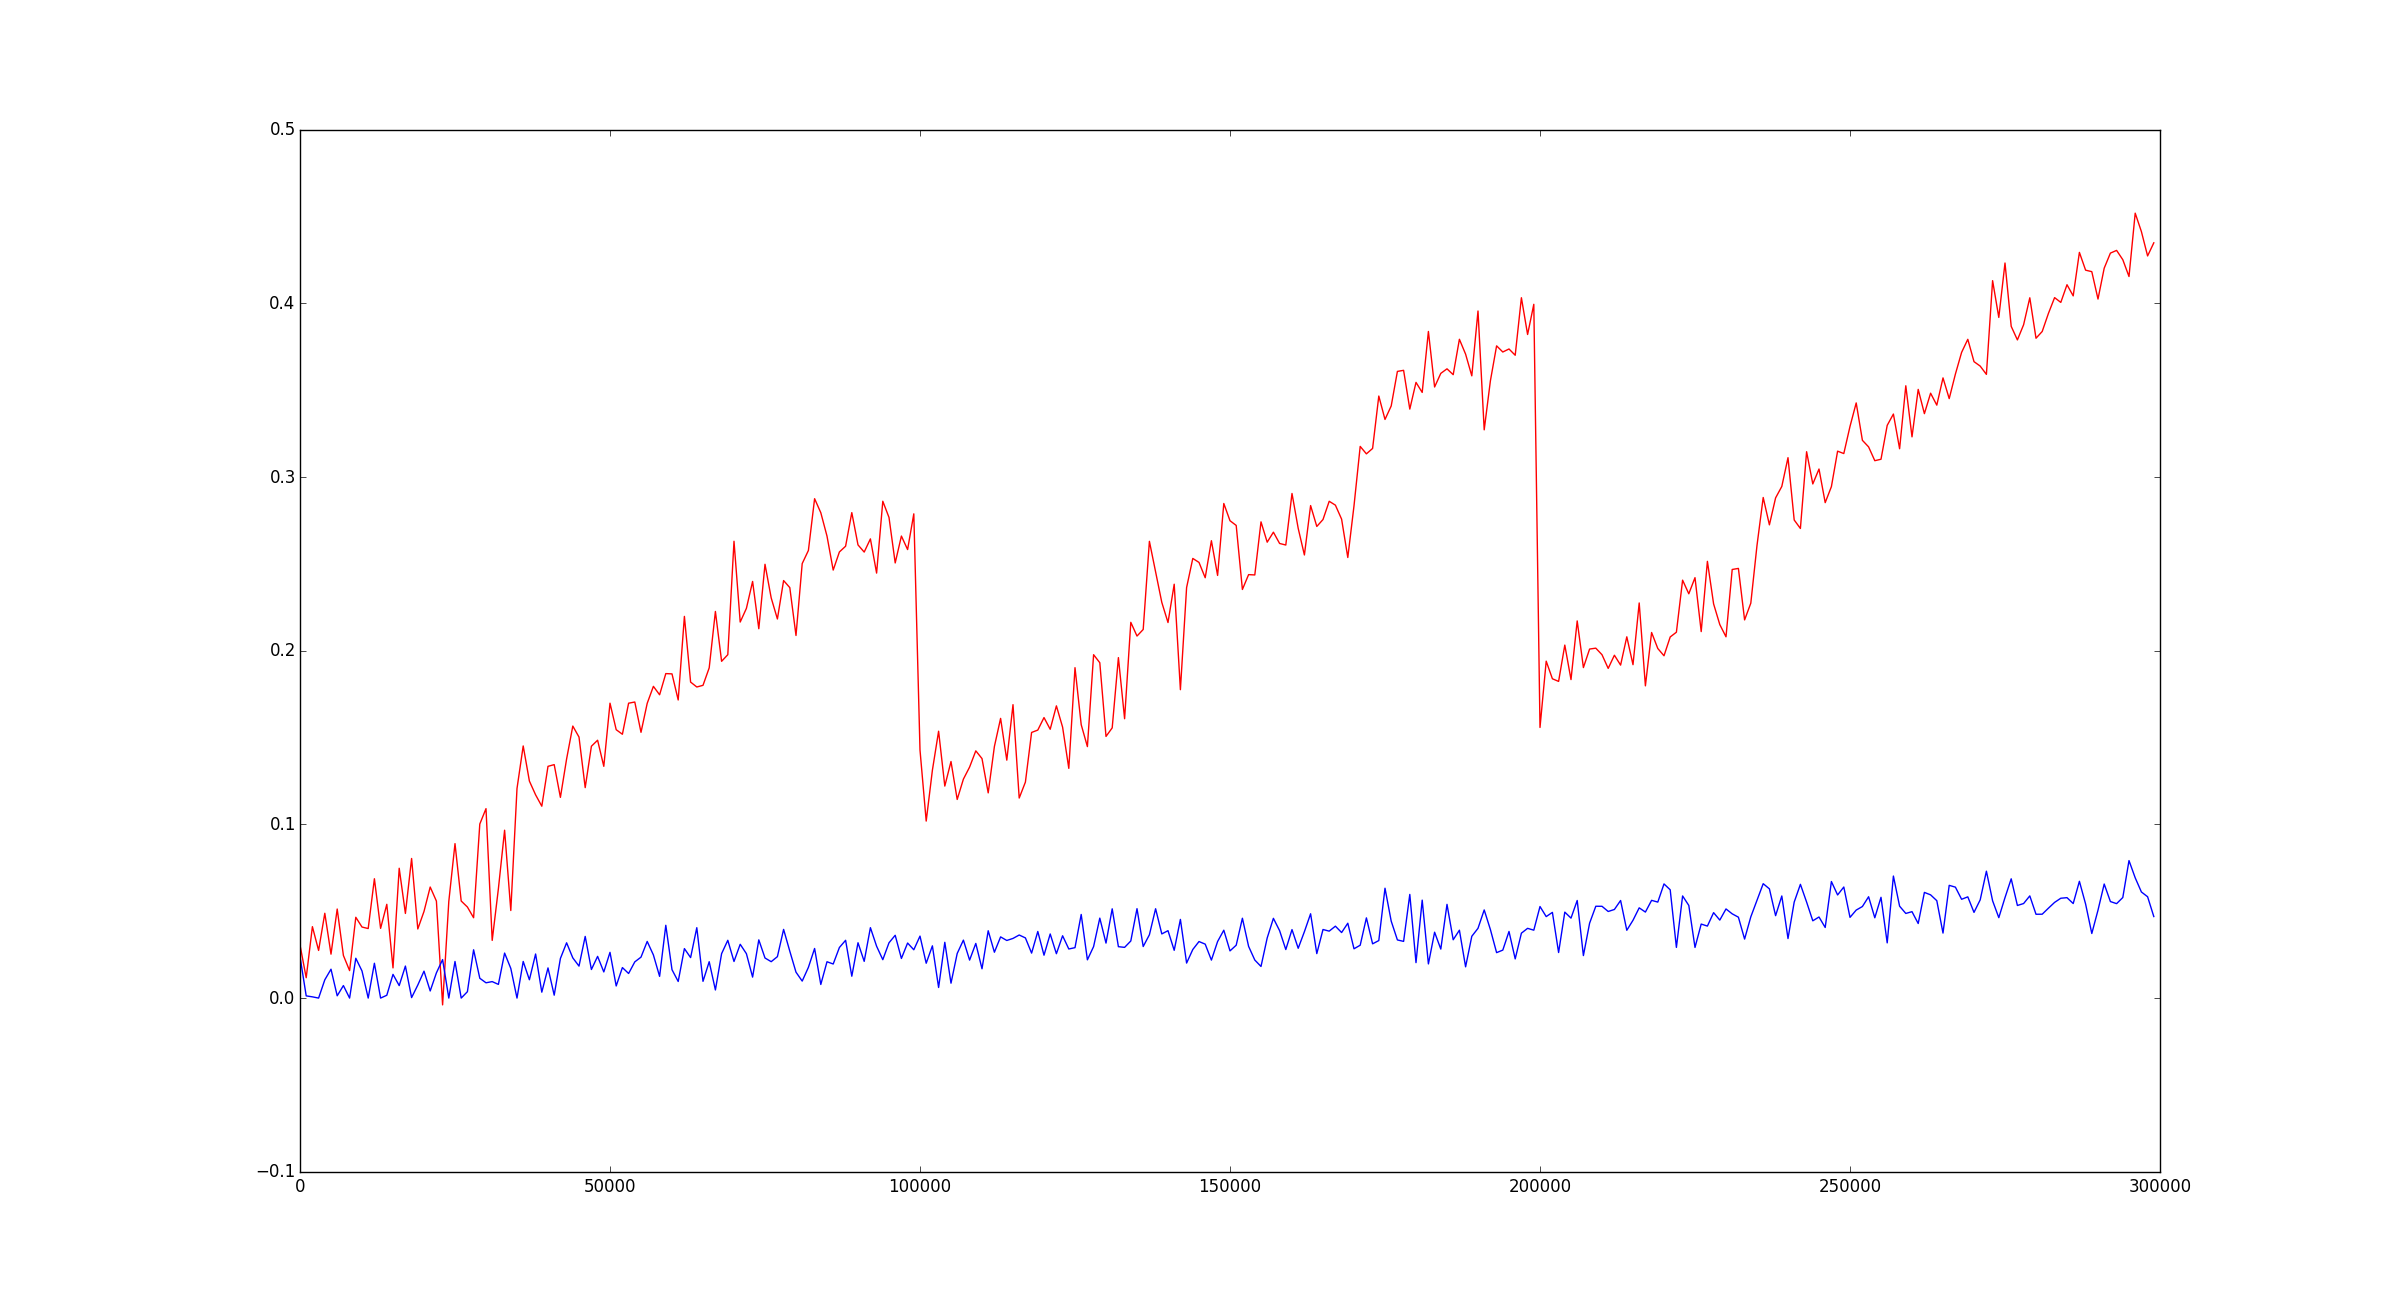
\includegraphics[scale=0.4]{firstfigure.png}
   \caption{\label{firstfigure} Training of the algorithm on cubes with $N=2$ that are 1 move away from being finished. X-axis represent the number of moves (and thus the number of updates of the parameters). Y-axis represent the moving average of success}
   \end{center}
\end{figure}

\section{Conclusion and future work}
This report presents the general Deep Q-learning algorithm and its adaptation for the Rubik's cube game. Despite the use of Curriculum Learning, the training of the model appears to be too slow ; it seems irealistic to have a Q-function that gives a good policy for the Rubik's cube with $N=3$ or more. We think that Deep Q-learning is not very appropriate for the Rubik's cube game as the neural network will have much troubles to generalize the patterns between the colors and the different faces and it can get easily lost in the exploration because the reward is only given at the end. Maybe is Deep Q-learning more approriate for problems where the environment is stochastic, such as the one in some games of \cite{deepmind}.

In order to tackle the problem of generalisation among faces and colors, a future idea is to design a network that does not make distinction between the orientation of the faces and between the permutation of the colors. We believe that this could help to learn faster.

\section{Acknowledgement}
The authors would like to thank the developers of Theano and Blocks.


\bibliographystyle{plain}
\bibliography{biblio}
\end{document}
